\section{NODE SOFTWARE}

\subsection{Description of the implementation}

The system extends the functionality of the Mbed-OS \acrshort{lorawan} example provided by the teachers, in which an event-queue is provided. This example is developed using Mbed-OS 6.16.0.

This event-queue provides an asynchronous event dispatcher, in this case for \acrshort{lorawan} events. And, for any event that happens in the system, a callback will be done to process that situation. This working can be seen in the next figure.

\begin{figure}[H]
    \centering
    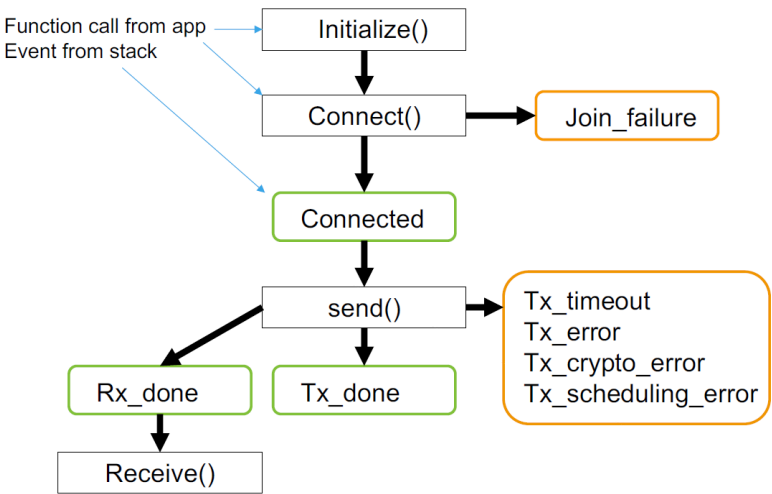
\includegraphics[width=0.6\textwidth]{images/4/event-queue.png}
    \caption{EventQueue process\cite{SensorNetworksProject1_slides_2024}}
    \label{fig:events}
\end{figure}

The solution is implemented by extending the previous event-queue. This event queue will detect possible TX windows in the \acrshort{lorawan} PHY layer and create an event to send a new message with data regarding the measurements of the plant sensors. These sensors are: 
GPS, brightness, soil moisture, humidity, temperature, linear acceleration, RGB data and led status.

To obtain this data, measurement threads are changed from the previous project, these threads are now independent and read new values each 5 seconds, storing the data in a mutex-controlled structure. This structure is later used when the \acrshort{lorawan} stack detects a possible transmitting window.

The threads defined for the solution are:
\begin{itemize}
    \item Main thread with the event-queue.
    \item I2C thread.
    \item GPS thread.
\end{itemize}
\subsection{Modules}
The modules used for this project are mainly the same from the previous course project, with the only exception being a new module to allocate the shared data for the communication between threads.

The module are also used by the same threads:
\begin{itemize}
    \item The I2C thread communicates with the accelerometer, temperature \& humidity and the color module.
    \item The GPS thread controls only the GPS module.
\end{itemize}

\clearpage
\subsection{Threads and communication design} % Comentar los cambios realizados

\acrshort{lorawan} is used, which analyzes a possible transmitting window for the next message. Because of this, a method is needed that ensures the maximum utilization of these windows without depending on the main thread. The final design for this can be seen in the next figure.

\begin{figure}[H]
    \centering
    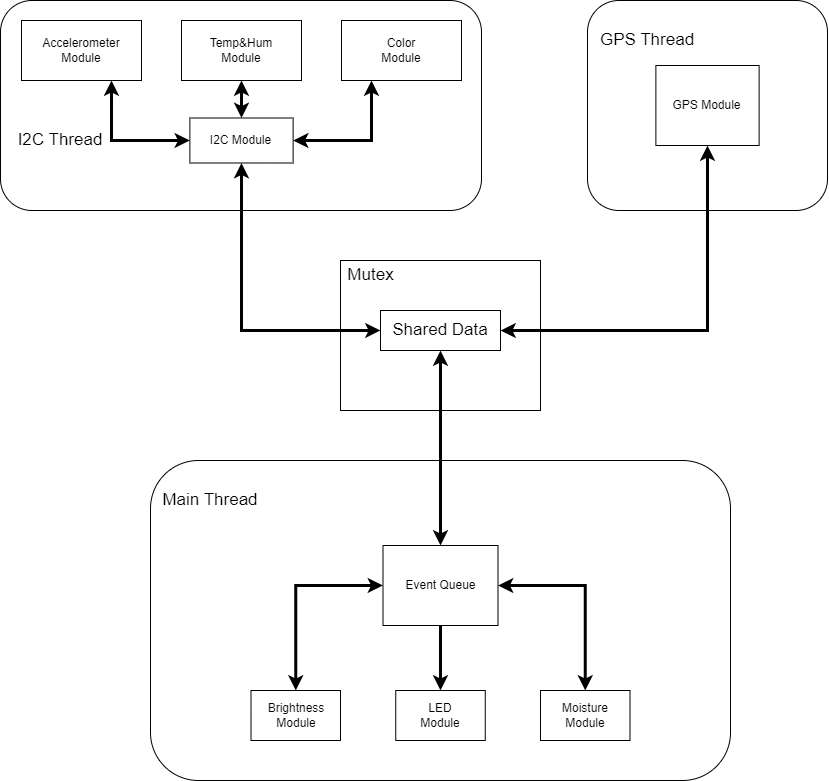
\includegraphics[width=0.85\textwidth]{images/4/Modules.png}
    \caption{Final module design for the system}
    \label{fig:modules}
\end{figure}
In the previous project, the approach was having the main thread controlling the execution of the measuring threads with signals. In this project, that won't work because the main thread is controlled by the event-queue. 
To solve this and taking into account the best-effort nature of the system, the decision was to make the measuring threads run independently of the main thread, waking themself up every \texttt{N} seconds. 

The communication between the measuring threads and the main thread had to be redone as well, as in the previous project used an intermediate queue. In this system that could create problems in the next events:
\begin{itemize}
    \item The system doesn't control the time between readings of the data, so there's a possibility of filling of the queue.
    \item The system only focuses on sending the last measurements possible for each sensor, so there's no need for previous data that isn't processed.
\end{itemize}

To solve all this situation, the communication was reduced to a shared structure that contains all the necessary data that is going to be sent through \acrshort{lorawan}. The access to this common structure is done using a Mbed-OS mutex, that ensures the protection of the data, allowing access to one thread at a time.

This structure is designed to be directly sent to the \acrshort{lorawan} software stack, so it's designed as a network frame. The structure is presented in the \hyperref[appendixA]{appendix} and it's explained in the next chapters.
\subsection{Frame design}

The frame that is sent as payload in the application level of \acrshort{lorawan} is presented in the next table.
\begin{table}[H]
    \centering
    \begin{bytefield}[bitwidth=1.45em]{30}
        \bitheader{0,1,29} \\
        \bitbox{1}{\tiny H \\D \\R} & \bitbox{29}{Message payload}
     \end{bytefield}
    \caption{Frame structure in bytes, with the header and the message payload}
\end{table}

It contains two main parts:
\begin{itemize}
    \item \textbf{The header}: this byte is defined as an advanced implementation, and is explained in the next chapter, but it provides support for message types, versions and led state.
    \item \textbf{The payload}: this structure of 29 bytes contains the data. And the content varies depending on the message type. But the system mainly uses the measurement report type, which contains all the sensor data to cover the requirements of the project. This type is presented in the next table.
\end{itemize}
\begin{table}[H]
    \centering
    \begin{bytefield}[bitwidth=1.35em]{32}
        \bitheader{0-31} \\
        \wordbox{1}{Latitude} \\
        \wordbox{1}{Longitude} \\
        \bitbox{16}{Altitude} & \bitbox{16}{Clear} \\
        \bitbox{16}{Red} & \bitbox{16}{Green} \\
        \bitbox{16}{Blue} & \bitbox{16}{Temperature} \\
        \bitbox{10}{Humidity (\texttt{10b})} & \bitbox{14}{X\_Acc (\texttt{14b})} & \bitbox{8}{Light (\texttt{MS 8b})}\\
        \bitbox{2}{\tiny Light(\texttt{2b})} & \bitbox{14}{Y\_Acc (\texttt{14b})} & \bitbox{10}{Moisture (\texttt{10b})} & \bitbox{6}{Z\_Acc (\texttt{MS 6b})}\\
        \bitbox{8}{Z\_Acc (\texttt{LS 8b})} & \bitbox{24}[bgcolor=lightgray]{}\\
     \end{bytefield}
    \caption{Measurement report structure}
\end{table}

All the data is sent as \textit{LITTLE ENDIAN}, and for each data the format was defined taking into account the constraint of the \texttt{29 Bytes}. The format for the measurement report data is:

\begin{enumerate}
    \item \textbf{Latitude \& Longitude }: The latitude and the longitude are transmitted as the whole signed float value (\texttt{4 Bytes} each), as any trunking of the value could potentially mean errors of several kilometers.
    \item \textbf{Altitude}: For the altitude, an unsigned \texttt{16 bit} integer value is sent to represent the altitude in meters above the sea level. This is because the minimum for this project is around $700m$ above sea level (Madrid city).
    \item \textbf{RGB Values}: The RGB Values are sent as raw data from the sensor, as unsigned \texttt{16 bit} values. This is done for all the sensor values which are: clear, read, green and blue, that means \texttt{8 Bytes} for the color data.
    \item \textbf{Temperature}: The Temperature is still sent as raw data from the sensor, as a signed \texttt{16 bit} integer. This means that the processing to obtain the degrees value must be done in the network server.
    \item \textbf{Humidity}: Up to this point, all the previous values where divisible by a whole \texttt{Byte}, but the message had already used 20 Bytes, and there was still the acceleration, humidity, light and soil moisture values that needed to be 
    send in \texttt{9 Bytes}. To solve this, a encoding was defined for the humidity, light and moisture values to only use \texttt{10 bits}. This design is part of the problems found chapter.
    \item \textbf{X\_Acc}: The acceleration values are sent as they come from the sensor, transmitting the whole \texttt{14 bits} of each axis.
    \item \textbf{Light}: The percentage value is transmitted using the same encoding for the humidity and soil moisture values in \texttt{10 bits}.
    \item \textbf{Y\_Acc}: The Y-axis acceleration \texttt{14 bit} signed value.
    \item \textbf{Soil Moisture}: The percentage value is transmitted using the same encoding for the humidity and light values in \texttt{10 bits}.
    \item \textbf{Z\_Acc}: The Z-axis acceleration \texttt{14 bit} signed value.
\end{enumerate}

As the whole message with the header uses the \texttt{30 Byte} limit of the \acrshort{lorawan} stack, no padding was used.

